\documentclass[tikz,border=10pt]{standalone}
\begin{document}
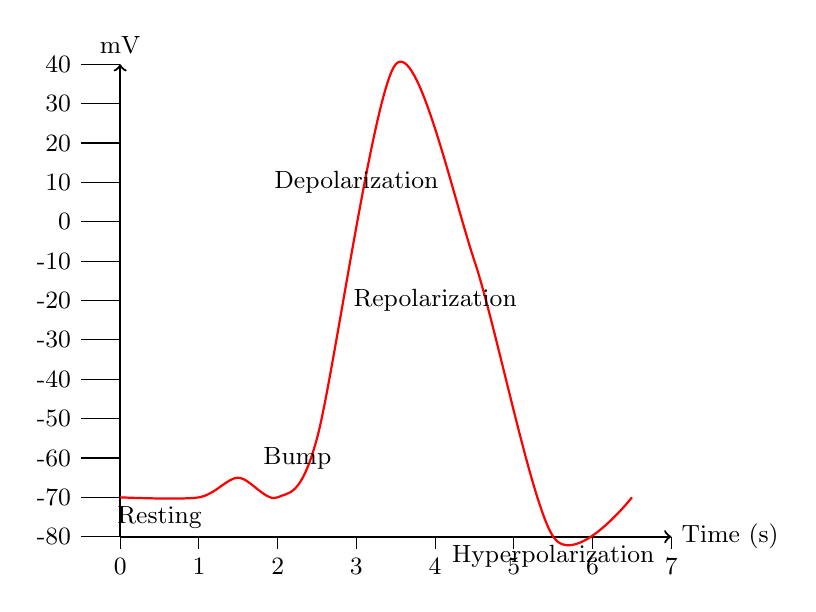
\begin{tikzpicture}[font=\small, xscale=1, yscale=0.05]
  % Draw axes:
  % The x-axis (time) is drawn along the bottom.
  \draw[->, thick] (0,-80) -- (7,-80) node[right] {Time (s)};
  % The y-axis (voltage in mV) is drawn on the left.
  \draw[->, thick] (0,-80) -- (0,40) node[above] {mV};

  % Draw y-axis ticks and labels (in mV)
  \foreach \y in {-80,-70,-60,-50,-40,-30,-20,-10,0,10,20,30,40} {
    \draw (0,\y) -- (-0.5,\y) node[left] {\y};
  }
  % Draw x-axis ticks (time in seconds)
  \foreach \x in {0,1,2,3,4,5,6,7} {
    \draw (\x,-80) -- (\x,-83) node[below] {\x};
  }

  % Plot the action potential waveform with a threshold bump:
  % Coordinates are given as (time in s, voltage in mV)
  \draw[thick, red, smooth] plot coordinates {
    (0, -70)     % resting potential at t=0
    (1, -70)     % still at rest
    (1.5, -65)   % a small bump (pre-threshold bump)
    (2, -70)     % return to rest before threshold
    (2.5, -55)   % threshold reached (-55 mV)
    (3.5, 40)    % peak depolarization (+40 mV)
    (4.5, -10)   % repolarization phase (-10 mV)
    (5.5, -80)   % hyperpolarization (-80 mV)
    (6.5, -70)   % return to resting potential (-70 mV)
  };

  % Optional: Add phase labels near the waveform
  \node at (0.5, -75) {Resting};
  \node at (2.25, -60) {Bump};
  \node at (3, 10) {Depolarization};
  \node at (4, -20) {Repolarization};
  \node at (5.5, -85) {Hyperpolarization};

\end{tikzpicture}
\end{document}